\documentclass[tikz,border=10pt]{standalone}
\usepackage{amsmath}
\usepackage[T1]{fontenc}
\usepackage{tikz}
\usetikzlibrary{positioning,arrows.meta,backgrounds,fit,calc}

% =====================================================================
%  Transconvolución 2D (Deconvolución)
%  Standalone, compilable. To embed in the thesis, copy the
%  \begin{tikzpicture}...\end{tikzpicture} block into a figure and
%  load: \usetikzlibrary{positioning,arrows.meta,backgrounds,fit,calc}
% =====================================================================

\definecolor{cblue}{RGB}{31,90,150}
\definecolor{cbluefill}{RGB}{225,236,247}
\definecolor{cgreen}{RGB}{40,120,55}
\definecolor{cgreenfill}{RGB}{231,243,228}
\definecolor{cpurple}{RGB}{95,50,135}
\definecolor{cpurplefill}{RGB}{243,238,248}
\definecolor{clightpurple}{RGB}{249,247,252}
\definecolor{cnavy}{RGB}{20,45,90}

\begin{document}
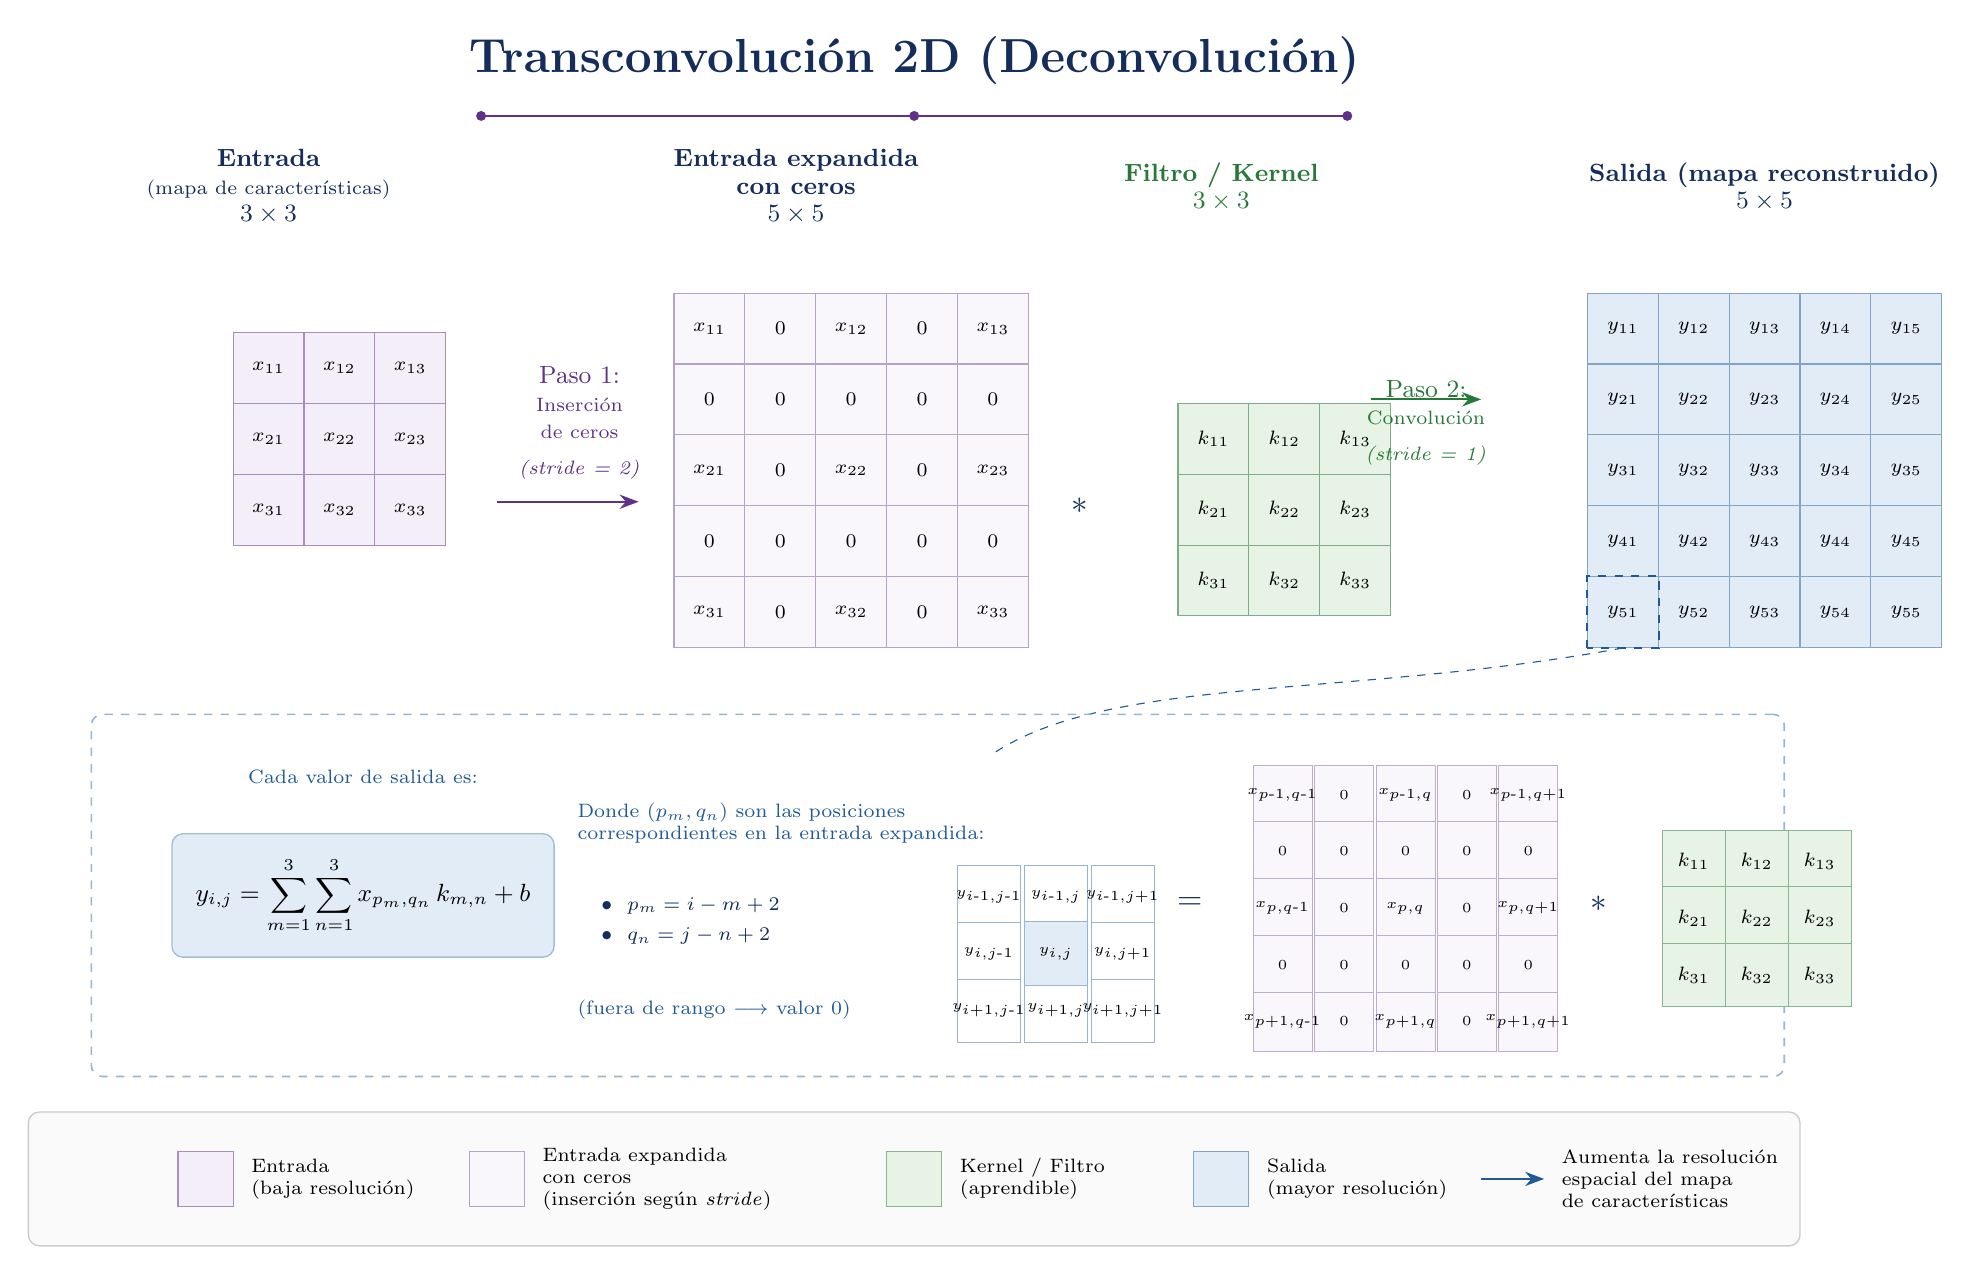
\begin{tikzpicture}[
  font=\small,
  >={Stealth[length=2.4mm]},
  cellP/.style={minimum size=9mm, draw=cpurple!55, line width=0.4pt, fill=cpurplefill, anchor=center},
  cellPe/.style={minimum size=9mm, draw=cpurple!45, line width=0.4pt, fill=clightpurple, anchor=center},
  cellG/.style={minimum size=9mm, draw=cgreen!60, line width=0.4pt, fill=cgreenfill, anchor=center},
  cellB/.style={minimum size=9mm, draw=cblue!55, line width=0.4pt, fill=cbluefill, anchor=center}
]

% ===================== TITLE =====================
\node[cnavy] at (9.5,7.6) {\bfseries\LARGE Transconvolución 2D (Deconvolución)};
\draw[cpurple, line width=1pt] (4.0,6.9)--(15.0,6.9);
\fill[cpurple] (4.0,6.9) circle (1.8pt); \fill[cpurple] (9.5,6.9) circle (1.8pt); \fill[cpurple] (15.0,6.9) circle (1.8pt);

% ===================== INPUT 3x3 =====================
\node[cnavy, align=center] at (1.3,6.0) {\bfseries Entrada\\[-1pt]\normalfont\scriptsize (mapa de características)\\[-1pt]$3\times3$};
\foreach \r in {1,2,3}{ \foreach \c in {1,2,3}{
  \pgfmathtruncatemacro{\rr}{\r}\pgfmathtruncatemacro{\cc}{\c}
  \node[cellP] at ({0.4+\c*0.9},{4.6-\r*0.9}) {\scriptsize$x_{\rr\cc}$};
}}

% step 1 arrow
\node[cpurple, align=center] at (5.25,3.0) {Paso 1:\\[-1pt]\scriptsize Inserción\\[-1pt]\scriptsize de ceros\\[2pt]\scriptsize\textit{(stride = 2)}};
\draw[cpurple,->,line width=0.7pt] (4.2,2.0)--(6.0,2.0);

% ===================== EXPANDED 5x5 =====================
\node[cnavy, align=center] at (8.0,6.0) {\bfseries Entrada expandida\\[-1pt]\bfseries con ceros\\[-1pt]$5\times5$};
% content: x where odd-odd, else 0
\foreach \r in {1,...,5}{ \foreach \c in {1,...,5}{
  \pgfmathtruncatemacro{\ro}{Mod(\r,2)}\pgfmathtruncatemacro{\co}{Mod(\c,2)}
  \pgfmathtruncatemacro{\xi}{(\r+1)/2}\pgfmathtruncatemacro{\xj}{(\c+1)/2}
  \ifnum\ro=1 \ifnum\co=1
     \node[cellPe] at ({6.0+\c*0.9},{5.1-\r*0.9}) {\scriptsize$x_{\xi\xj}$};
  \else
     \node[cellPe] at ({6.0+\c*0.9},{5.1-\r*0.9}) {\scriptsize$0$};
  \fi\else
     \node[cellPe] at ({6.0+\c*0.9},{5.1-\r*0.9}) {\scriptsize$0$};
  \fi
}}

% convolution symbol
\node[cnavy] at (11.6,1.95) {\large $*$};

% ===================== KERNEL 3x3 =====================
\node[cgreen, align=center] at (13.4,6.0) {\bfseries Filtro / Kernel\\[-1pt]$3\times3$};
\foreach \r in {1,2,3}{ \foreach \c in {1,2,3}{
  \pgfmathtruncatemacro{\rr}{\r}\pgfmathtruncatemacro{\cc}{\c}
  \node[cellG] at ({12.4+\c*0.9},{3.7-\r*0.9}) {\scriptsize$k_{\rr\cc}$};
}}

% step 2 arrow
\node[cgreen, align=center] at (16.0,3.0) {Paso 2:\\[-1pt]\scriptsize Convolución\\[2pt]\scriptsize\textit{(stride = 1)}};
\draw[cgreen,->,line width=0.7pt] (15.3,3.3)--(16.7,3.3);

% ===================== OUTPUT 5x5 =====================
\node[cnavy, align=center] at (20.3,6.0) {\bfseries Salida (mapa reconstruido)\\[-1pt]$5\times5$};
\foreach \r in {1,...,5}{ \foreach \c in {1,...,5}{
  \pgfmathtruncatemacro{\rr}{\r}\pgfmathtruncatemacro{\cc}{\c}
  \node[cellB] (O\r\c) at ({17.6+\c*0.9},{5.1-\r*0.9}) {\scriptsize$y_{\rr\cc}$};
}}
% dashed highlight on y51
\draw[cblue, dashed, line width=0.7pt] (O51.south west) rectangle (O51.north east);

% dashed projection from y51 down to detail panel
\draw[cblue, dashed, line width=0.4pt] (O51.south) .. controls (15,-0.5) and (12,-0.2) .. (10.5,-1.2);

% ===================== DETAIL PANEL =====================
\node[draw=cblue!45, dashed, rounded corners, line width=0.6pt,
      minimum width=21.5cm, minimum height=4.6cm] at (9.8,-3.0) {};

% formula box
\node[draw=cblue!40, fill=cbluefill, rounded corners, inner sep=3mm, line width=0.5pt]
  (fbox) at (2.5,-3.0) {$\displaystyle y_{i,j}=\sum_{m=1}^{3}\sum_{n=1}^{3} x_{p_m,q_n}\,k_{m,n}+b$};
\node[cblue, anchor=south, font=\scriptsize] at (2.5,-1.7) {Cada valor de salida es:};

% (p_m,q_n) text
\node[cblue, align=left, font=\scriptsize, anchor=north west] at (5.1,-1.7)
  {Donde $(p_m,q_n)$ son las posiciones\\ correspondientes en la entrada expandida:};
\node[cnavy, align=left, font=\scriptsize, anchor=north west] at (5.4,-2.9)
  {$\bullet\ \ p_m = i-m+2$\\[3pt]$\bullet\ \ q_n = j-n+2$};
\node[cblue, font=\scriptsize, anchor=north west] at (5.1,-4.2)
  {(fuera de rango $\longrightarrow$ valor 0)};

% small y-neighbourhood 3x3
\foreach \r in {1,2,3}{ \foreach \c in {1,2,3}{
  \node[minimum size=8mm, draw=cblue!45, line width=0.3pt, fill=white]
    (N\r\c) at ({9.6+\c*0.85},{-2.3-\r*0.72}) {};
}}
% highlight central cell
\fill[cbluefill] (N22.south west) rectangle (N22.north east);
\draw[cblue!45, line width=0.3pt] (N22.south west) rectangle (N22.north east);
\node[font=\tiny] at (N11) {$y_{i\text{-}1,j\text{-}1}$};
\node[font=\tiny] at (N12) {$y_{i\text{-}1,j}$};
\node[font=\tiny] at (N13) {$y_{i\text{-}1,j\text{+}1}$};
\node[font=\tiny] at (N21) {$y_{i,j\text{-}1}$};
\node[font=\tiny] at (N22) {$y_{i,j}$};
\node[font=\tiny] at (N23) {$y_{i,j\text{+}1}$};
\node[font=\tiny] at (N31) {$y_{i\text{+}1,j\text{-}1}$};
\node[font=\tiny] at (N32) {$y_{i\text{+}1,j}$};
\node[font=\tiny] at (N33) {$y_{i\text{+}1,j\text{+}1}$};

\node[cnavy] at (13.0,-3.1) {\large $=$};

% expanded 5x5 neighbourhood (with x_{p..} and zeros)
\foreach \r in {1,...,5}{ \foreach \c in {1,...,5}{
  \pgfmathtruncatemacro{\ro}{Mod(\r,2)}\pgfmathtruncatemacro{\co}{Mod(\c,2)}
  \node[minimum size=7.5mm, draw=cpurple!40, line width=0.3pt, fill=clightpurple]
    (E\r\c) at ({13.4+\c*0.78},{-1.0-\r*0.72}) {};
}}
% fill labels: odd-odd cells get x_{p..}, others 0
\node[font=\tiny] at (E11) {$x_{p\text{-}1,q\text{-}1}$};
\node[font=\tiny] at (E13) {$x_{p\text{-}1,q}$};
\node[font=\tiny] at (E15) {$x_{p\text{-}1,q\text{+}1}$};
\node[font=\tiny] at (E31) {$x_{p,q\text{-}1}$};
\node[font=\tiny] at (E33) {$x_{p,q}$};
\node[font=\tiny] at (E35) {$x_{p,q\text{+}1}$};
\node[font=\tiny] at (E51) {$x_{p\text{+}1,q\text{-}1}$};
\node[font=\tiny] at (E53) {$x_{p\text{+}1,q}$};
\node[font=\tiny] at (E55) {$x_{p\text{+}1,q\text{+}1}$};
\foreach \rc in {12,14,21,22,23,24,25,32,34,41,42,43,44,45,52,54}{
  \node[font=\tiny] at (E\rc) {$0$};
}

\node[cnavy] at (18.2,-3.1) {\large $*$};

% kernel 3x3 in panel
\foreach \r in {1,2,3}{ \foreach \c in {1,2,3}{
  \pgfmathtruncatemacro{\rr}{\r}\pgfmathtruncatemacro{\cc}{\c}
  \node[minimum size=8mm, draw=cgreen!55, line width=0.3pt, fill=cgreenfill]
    at ({18.6+\c*0.8},{-1.85-\r*0.72}) {\scriptsize$k_{\rr\cc}$};
}}

% ===================== LEGEND =====================
\node[draw=black!20, fill=black!2, rounded corners, line width=0.5pt,
      minimum width=22.5cm, minimum height=1.7cm] at (9.5,-6.6) {};
\node[minimum size=7mm, draw=cpurple!55, fill=cpurplefill] (g1) at (0.5,-6.6) {};
\node[right=1mm of g1, align=left, font=\scriptsize] {Entrada\\(baja resolución)};
\node[minimum size=7mm, draw=cpurple!45, fill=clightpurple] (g2) at (4.2,-6.6) {};
\node[right=1mm of g2, align=left, font=\scriptsize] {Entrada expandida\\con ceros\\(inserción según \textit{stride})};
\node[minimum size=7mm, draw=cgreen!55, fill=cgreenfill] (g3) at (9.5,-6.6) {};
\node[right=1mm of g3, align=left, font=\scriptsize] {Kernel / Filtro\\(aprendible)};
\node[minimum size=7mm, draw=cblue!55, fill=cbluefill] (g4) at (13.4,-6.6) {};
\node[right=1mm of g4, align=left, font=\scriptsize] {Salida\\(mayor resolución)};
\draw[cblue,->,line width=0.8pt] (16.7,-6.6)--(17.5,-6.6);
\node[anchor=west, align=left, font=\scriptsize] at (17.6,-6.6) {Aumenta la resolución\\espacial del mapa\\de características};

\end{tikzpicture}
\end{document}
